\documentclass[aspectratio=169,xcolor={dvipsnames,table}]{beamer}
\usepackage[no-math,deluxe,haranoaji]{luatexja-preset}
\renewcommand{\kanjifamilydefault}{\gtdefault}
\renewcommand{\emph}[1]{{\upshape\bfseries #1}}
\usetheme{metropolis}
\metroset{block=fill}
\setbeamertemplate{navigation symbols}{}
\setbeamertemplate{blocks}[rounded][shadow=false]
\usecolortheme[rgb={0.7,0.2,0.2}]{structure}
%%%%%%%%%%%%%%%%%%%%%%%%%%
%% Change alert block colors
%%% 1- Block title (background and text)
\setbeamercolor{block title alerted}{fg=mDarkTeal, bg=mLightBrown!45!yellow!45}
\setbeamercolor{block title example}{fg=magenta!10!black, bg=mLightGreen!70}
%%% 2- Block body (background)
\setbeamercolor{block body alerted}{bg=mLightBrown!25}
\setbeamercolor{block body example}{bg=mLightGreen!15}
%%%%%%%%%%%%%%%%%%%%%%%%%%%
%%%%%%%%%%%%%%%%%%%%%%%%%%%
%% さまざまなアイコン
%%%%%%%%%%%%%%%%%%%%%%%%%%%
%\usepackage{fontawesome}
\usepackage{fontawesome5}
\usepackage{figchild}
\usepackage{twemojis}
\usepackage{utfsym}
\usepackage{bclogo}
\usepackage{marvosym}
\usepackage{fontmfizz}
\usepackage{pifont}
\usepackage{phaistos}
\usepackage{worldflags}
\usepackage{jigsaw}
\usepackage{tikzlings}
\usepackage{tikzducks}
\usepackage{scsnowman}
\usepackage{epsdice}
\usepackage{halloweenmath}
\usepackage{svrsymbols}
\usepackage{countriesofeurope}
\usepackage{tipa}
\usepackage{manfnt}
%%%%%%%%%%%%%%%%%%%%%%%%%%%
\usepackage{tikz}
\usetikzlibrary{calc,patterns,decorations.pathmorphing,backgrounds}
\usepackage{tcolorbox}
\usepackage{tikzpeople}
\usepackage{circledsteps}
\usepackage{xcolor}
\usepackage{amsmath}
\usepackage{booktabs}
\usepackage{chronology}
\usepackage{signchart}
%%%%%%%%%%%%%%%%%%%%%%%%%%%
%% 場合分け
%%%%%%%%%%%%%%%%%%%%%%%%%%%
\usepackage{cases}
%%%%%%%%%%%%%%%%%%%%%%%%%%
\usepackage{pdfpages}
%%%%%%%%%%%%%%%%%%%%%%%%%%%
%% 音声リンク表示
\newcommand{\myaudio}[1]{\href{#1}{\faVolumeUp}}
%%%%%%%%%%%%%%%%%%%%%%%%%%
%% \myAnch{<名前>}{<色>}{<テキスト>}
%% 指定のテキストを指定の色の四角枠で囲み, 指定の名前をもつTikZの
%% ノードとして出力する. 図には remember picture 属性を付けている
%% ので外部から参照可能である.
\newcommand*{\myAnch}[3]{%
  \tikz[remember picture,baseline=(#1.base)]
    \node[draw,rectangle,line width=1pt,#2] (#1) {\normalcolor #3};
}
%%%%%%%%%%%%%%%%%%%%%%%%%%
%% \myEmph コマンドの定義
%%%%%%%%%%%%%%%%%%%%%%%%%%
%\newcommand{\myEmph}[3]{%
%    \textbf<#1>{\color<#1>{#2}{#3}}%
%}
\usepackage{xparse} % xparseパッケージの読み込み
\NewDocumentCommand{\myEmph}{O{} m m}{%
    \def\argOne{#1}%
    \ifx\argOne\empty
        \textbf{\color{#2}{#3}}% オプション引数が省略された場合
    \else
        \textbf<#1>{\color<#1>{#2}{#3}}% オプション引数が指定された場合
    \fi
}
%%%%%%%%%%%%%%%%%%%%%%%%%%%
%%%%%%%%%%%%%%%%%%%%%%%%%%%
%% 文末の上昇イントネーション記号 \myRisingPitch
%% 通常のイントネーション \myDownwardPitch
%% https://note.com/dan_oyama/n/n8be58e8797b2
%%%%%%%%%%%%%%%%%%%%%%%%%%%
\newcommand{\myRisingPitch}{
\begin{tikzpicture}[scale=0.3,baseline=0.3]
\draw[->,>=stealth] (0,0) to[bend right=45] (1,1);
\end{tikzpicture}
}
\newcommand{\myDownwardPitch}{
\begin{tikzpicture}[scale=0.3,baseline=0.3]
\draw[->,>=stealth] (0,1) to[bend left=45] (1,0);
\end{tikzpicture}
}
%%%%%%%%%%%%%%%%%%%%%%%%%%%%
%\AtBeginSection[%
%]{%
%  \begin{frame}[plain]\frametitle{授業の流れ}
%     \tableofcontents[currentsection]
%   \end{frame}%
%}

\usepackage{pxrubrica}
\usetikzlibrary{tikzmark}
%%%%%%%%%%%%%%%%%%%%%%%%%%%
\title{English is fun.}
\subtitle{I know where she was born.}
\author{}
\institute[]{}
\date[]

%%%%%%%%%%%%%%%%%%%%%%%%%%%%
%% TEXT
%%%%%%%%%%%%%%%%%%%%%%%%%%%%
\begin{document}


\begin{frame}[plain]
  \titlepage
\end{frame}


\section*{授業の流れ}
\begin{frame}[plain]
  \frametitle{授業の流れ}
  \tableofcontents
\end{frame}

\section{復習}
\subsection{that}
%%%%%%%%%%%%%%%%%%%%%%%%%%%%%%%%%%%%%%%%%%%%%
\begin{frame}[plain]{S $+$ V \fbox{that s $+$ v}}
\large
\begin{enumerate}
 \item<1-> I know George.\hfill{\scriptsize Georgeは目的語(O)}
 \item<2-> I know the fact.\hfill{\scriptsize fact \textipa{/f\'\ae kt/} 事実}
 \item<3-> I know \fbox{that she is kind}.\hfill{}{\small \textbf{S} $+$ \textbf{V}\,\,\fbox{that s $+$ v}\,($=$O)}
 \item<4-> I know she is kind.

\end{enumerate}
\mbox{}\hfill{\scriptsize \myaudio{./audio/055_indirect_question_01.mp3}}

\begin{block}<5->{Topics for Today}\small
\begin{itemize}\setbeamertemplate{items}[square]\small
 \item   \Circled[fill color = white]{ that  s $+$ v }\,は「〜ということ」という意味
 \item   \Circled[fill color = white]{ that s $+$ v }\,は全体で「名詞」の役割
 \item  \textbf{that}の品詞は\kenten{接続詞}です
 \item 接続詞の\textbf{that}は省略されることもあります
\end{itemize}
     \end{block}
\end{frame}
%%%%%%%%%%%%%%%%%%%%%%%%
\section{間接疑問文}
\subsection{一般動詞のとき}
\begin{frame}[plain]{間接疑問文}\large
 \begin{enumerate}
  \item \begin{enumerate}
	 \item<1-> She lives in Tokyo.
	 \item<2-> I know \visible<3->{\fbox{(that) she lives in Tokyo}.} 
	\end{enumerate}
  \item \begin{enumerate}
	 \item<4-> Where does she live?
	 \item<5-> I know \visible<6->{\fbox{where she lives}.}
	 \item<7-> *I know where does she live.\hfill{\scriptsize *は、まちがった英文につける記号}
	\end{enumerate}
 \end{enumerate}

\begin{block}<8->{Topics for Today}\small
 \begin{itemize}\setbeamertemplate{items}[square]
  \item 疑問詞ではじまる疑問文をほかの文(I knowなど)と組み合わせることができます\\
  \item このときI know \Circled[fill color=white]{ 疑問詞\tikzmark{indirect} S $+$ V \ldots\,\,}\,\,となります\\
\mbox{}\hfill{\scriptsize \tikzmark{teigi}これを\kenten{間接疑問文}といいます}  \item 間接疑問文ではdo, does, didを使いません
 \end{itemize}

\begin{tikzpicture}[remember picture,overlay]
 \visible<8->{\draw[<-] ([xshift=2pt,yshift=-4pt]pic cs:indirect) |- ([xshift=-2pt, yshift=2pt] pic cs:teigi);}
\end{tikzpicture}

\end{block}
\mbox{}\hfill{\scriptsize \myaudio{./audio/055_indirect_question_02.mp3}}
\end{frame}
%%%%%%%%%%%%%%%%%%%%%%%%%%%%%
\subsection{be動詞のとき}
\begin{frame}[plain]{be動詞のとき}
 \begin{enumerate}
  \item<1-> Where is the station?
  \item<2-> I know \visible<3->{\fbox{where the station is}.}
  \item<4-> *I know where is the station.
 \end{enumerate}

\begin{block}<5->{Topics for Today}\small
\begin{itemize}\setbeamertemplate{items}[square]\small
 \item be動詞が使われている疑問文も間接疑問文になります
 \item 語順は\Circled[fill color=white]{ 疑問詞 S $+$ V }となります
\end{itemize}
\hfill{\scriptsize 一般動詞でもbe動詞でも同じです}
\end{block}
\mbox{}\hfill{\scriptsize \myaudio{./audio/055_indirect_question_03.mp3}}

\end{frame}
%%%%%%%%%%%%%%%%%%%%%%%%%%%%%%%%%%%%%%%%%
\section{Exercises}
\begin{frame}[plain]{Exercises}
カッコ内から正しいほうを選びましょう%
\mbox{}\hfill{\scriptsize \myaudio{./audio/055_indirect_question_04.mp3}}

 \begin{enumerate}
  \item I know why ( \alt<2->{\Circled[outer color=Maroon]{she is}}{she is} / is she ) sad.
  \item Please tell me where ( \alt<3->{\Circled[outer color=Maroon]{you bought}}{you bought} / did you buy ) the book.\\%
\hfill{\scriptsize tell 人 $+$ ~「人に~を話す、教える」}
  \item I remember ( where did I see / \alt<4->{\Circled[outer color=Maroon]{when I saw}}{when I saw} ) the man.
  \item I have no idea what ( is this / \alt<5->{\Circled[outer color=Maroon]{this is}}{this is} ).%
\hfill{\scriptsize have no idea まったくわからない}
  \item Do you know how ( \alt<6->{\Circled[outer color=Maroon]{she felt}}{she felt} / did she feel ) then?\hfill{\scriptsize feel--felt--felt}
  \item He knows what ( color does she like / \alt<7->{\Circled[outer color=Maroon]{sport she likes}}{sport she likes} ).
 \item Do you know ( how many cars does she have / \alt<8->{\Circled[outer color=Maroon]{how many cars she has}}{how many cars she has}).
 \end{enumerate}
\end{frame}
%%%%%%%%%%%%%%%%%%%%%%%%%%%%%%
\begin{frame}[plain]{Exercises}\small

{\small 日本語の意味になるようカッコ内の語句を並べかえましょう。
文頭の語は大文字で始めてください}%
\mbox{}\hfill{\scriptsize \myaudio{./audio/055_indirect_question_05.mp3}}

 \begin{enumerate}
  \item {わたしはなぜ彼女が怒っているか理解している。}\\
( why / I / she / is / understand / angry ). \\
\visible<2->{I understand why she is angry.}
  \item {彼がゆうべどこへ行ったかかご存じですか。}\\
( where / know / do / went / he / you ) last night? \\
\visible<3->{Do you know where he went last night?}
  \item {わたしは彼らがいつパリへ行くか知らない。}\\
( know / they / go / I / to / don't / when / will ) Paris. \\
\visible<4->{I don't know when they will go to Paris.}
  \item {誕生日に何がほしいか教えてください。}\\
( your / you / me / want / tell / birthday / for / what ) \\
\visible<5->{Tell me what you want for your birthday.}

 \end{enumerate}
\end{frame}
%%%%%%%%%%%%%%%%%%%%%%%%%%%%%%%
\begin{frame}[plain]{Exercises}
\small
\begin{tcolorbox}[colframe=ForestGreen,
  colback=ForestGreen!10!white,
  colbacktitle=ForestGreen!40!white,
  coltitle=black, %fonttitle=\bfseries,
  before upper={\setlength{\parindent}{1.5em}},
  title=英文を読んで、問に答えましょう\hfill{\scriptsize \myaudio{./audio/055_indirect_question_06.mp3}}
]
Lily and Tom were at the \tikzmark{clue1}zoo.
Tom pointed at an animal and asked, ``Do you know what that is?''
Lily looked closely. ``I don't \tikzmark{clue2}remember what it's called, but it looks funny!''
Tom checked the sign. ``It's a capy\tikzmark{clue3}bara!''
Lily laughed. ``Now I understand why it looks familiar. I saw one on TV!''

Later, their teacher asked, ``Can you tell me which ani\tikzmark{clue5}mal you liked best?''
Tom grinned. ``The capybara! It looks just like my gran\tikzmark{clue4}dpa!''
\end{tcolorbox}
\visible<2->{\scriptsize 英文の内容とあっていればT、あっていなければFと答えましょう}
\vspace{-3pt}
\begin{enumerate}\scriptsize\setlength{\itemsep}{-2pt}
 \item<2-> TomとLilyは動物園にいった\tikzmark{q1}\hfill\visible<4->{T}
 \item<2-> Lilyは見た動物の名前をすぐにおもいだした\tikzmark{q2}\hfill\visible<6->{F}
 \item<2-> ふたりが見た動物はカンガルーだった\tikzmark{q3}\hfill\visible<8->{F}
 \item<2-> Tomはカピバラがおじいさんに似ているとおもった\tikzmark{q4}\hfill\visible<10->{T}
 \item<2-> 先生はお気に入りの食べ物についてたずねた\tikzmark{q5}\hfill\visible<12->{F}
\end{enumerate}
% 以下は選択肢を英語にしたもの
%\begin{enumerate}\scriptsize\setlength{\itemsep}{-2pt}
% \item<2-> Tom and Lily went to the zoo.\tikzmark{q1}\hfill\visible<4->{T}
% \item<2-> Lily immediately remembered the name of the animal.\tikzmark{q2}\hfill\visible<6->{F}
% \item<2-> The animal they saw was a kangaroo.\tikzmark{q3}\hfill\visible<8->{F}
% \item<2-> Tom thought the capybara looked like his grandfather.\tikzmark{q4}\hfill\visible<10->{T}
% \item<2-> Their teacher asked about their favorite food.\tikzmark{q5}\hfill\visible<12->{F}
%\end{enumerate}


\begin{tikzpicture}[remember picture,overlay]
 \visible<3->{\draw[<-] ([yshift=-2pt]pic cs:clue1) to ([xshift=2pt, yshift=2pt] pic cs:q1);}
 \visible<5->{\draw[<-] ([yshift=-2pt]pic cs:clue2) to[bend left] ([xshift=2pt, yshift=2pt] pic cs:q2);}
 \visible<7->{\draw[<-] ([yshift=-2pt]pic cs:clue3) to ([xshift=2pt, yshift=2pt] pic cs:q3);}
 \visible<9->{\draw[<-] ([yshift=-2pt]pic cs:clue4) to[bend left] ([xshift=2pt, yshift=2pt] pic cs:q4);}
 \visible<11->{\draw[<-] ([yshift=-2pt]pic cs:clue5) to[out=-90,in=0] ([xshift=2pt, yshift=2pt] pic cs:q5);}
\end{tikzpicture}
\end{frame}
%%%%%%%%%%%%%%%%%%%%%%%%%%%%%%%
\section{まとめ}

\begin{frame}[plain]
 
\begin{columns}[t]
%%%%%%%%%%%%%%%%%%%%%%%%%
 \begin{column}{.45\textwidth}  
\begin{enumerate}
 \item Where does he live?
 \item I know where he lives.
 \item[2'.] *I know where does he live.
\end{enumerate}
 \end{column}
%%%%%%%%%%%%%%%%%%%%%%
 \begin{column}{.45\textwidth}  
 \begin{enumerate}\setcounter{enumi}{2}
  \item What is this?
   \item Do you know what this is?
  \item[4'.] *Do you know what is this?
 \end{enumerate}
 \end{column}
%%%%%%%%%%%%%%%%%%%%%%%
\end{columns}

\begin{block}<2->{間接疑問文}\small
 \begin{itemize}\setbeamertemplate{items}[square]
  \item 疑問詞ではじまる疑問文をほかの文(I knowなど)と組み合わせることができます\\
  \item このときI know \Circled[fill color=white]{ 疑問詞\tikzmark{indirect} S $+$ V \ldots\,\,}\,\,となります\\
\mbox{}\hfill{\scriptsize \tikzmark{teigi}これを\kenten{間接疑問文}といいます}  \item 間接疑問文ではdo, does, didを使いません
 \end{itemize}

\begin{tikzpicture}[remember picture,overlay]
 \visible<2->{\draw[<-] ([xshift=2pt,yshift=-4pt]pic cs:indirect) |- ([xshift=-2pt, yshift=2pt] pic cs:teigi);}
\end{tikzpicture}
\end{block}
\mbox{}\hfill{\scriptsize \myaudio{./audio/055_indirect_question_07.mp3}}

\end{frame}
%%%%%%%%%%%%%%%%%%%%%%%%%%%%%%%
\begin{frame}[plain]
 \begin{enumerate}
  \item \begin{enumerate}
	 \item<1-> She was born in Tokyo.%
\mbox{}\hfill{\scriptsize \myaudio{./audio/055_indirect_question_08.mp3}}

	 \item<2-> I know \visible<3->{\textbf<3->{that} she was born in Tokyo.} 
	 \item<4-> I know she was born in Tokyo.
	\end{enumerate}
  \item \begin{enumerate}
	 \item<5-> \textbf<5->{Where} was she born?
	 \item<6-> I know \visible<7->{\textbf<7->{where} she was born.}
%	 \item<8-> *I know that where she was born.
	\end{enumerate}
 \end{enumerate}


\begin{block}<8->{Topics for Today}\small
I knowなどにほかの文を続けるとき、続ける文が
 \begin{enumerate}
  \item ふつうの文(She was born in Tokyo.)のとき
         \begin{itemize}\setbeamertemplate{items}[circle]
	   \item I know \textbf{that} she was born in Tokyo.のように\kenten{接続詞}\textbf{that}をもちいます
	  \item I know she was born in Tokyo.のように\textbf{that}が\kenten{省略}されることもあります
	  \end{itemize}
  \item \kenten{疑問詞}をもちいた疑問文(\textbf{Where} was she born?)のときは
        \begin{itemize}\setbeamertemplate{items}[circle]
	 \item I know where she was born.のように\,\,\Circled[fill color = white]{\,疑問詞 S $+$ V\,}\,\,を続けます
	 \item *I know where was she born.はまちがいです
	 \item *I know that where she was born.はまちがいです
	\end{itemize}
 \end{enumerate}
\end{block}
\end{frame}
%%%%%%%%%%%%%%%%%%%%%%%%%%%%
\end{document}
